\documentclass{article}

\usepackage{aistats2021_author_response}

\usepackage[utf8]{inputenc} % allow utf-8 input
\usepackage[T1]{fontenc}    % use 8-bit T1 fonts
\usepackage{hyperref}       % hyperlinks
\usepackage{url}            % simple URL typesetting
\usepackage{booktabs}       % professional-quality tables
\usepackage{amsfonts}       % blackboard math symbols
\usepackage{nicefrac}       % compact symbols for 1/2, etc.
\usepackage{microtype}      % microtypography
\usepackage{xcolor}         % define colors in text
\usepackage{xspace}         % fix spacing around commands
\usepackage{subfigure}
\usepackage{float}
\usepackage{graphicx}

\begin{document}

We sincerely thank the five reviewers for their valuable feedback.


\vspace{0.01in}

\textbf{\textcolor{blue}{Reviewer 6:}} We thank the reviewer for valuable comments. Our point-to-point response is as follows:\vspace{-5pt}

\textbf{Notations:} In Lemma 2, the notation $\bar{\nabla} f(.)$ corresponds to the the average of $\nabla f(\theta_{r,i})$ over all clients $i \in [n]$. This is defined in the appendix (page 6) but will be clarified in the main.
The subscript $t$ will be changed to $r$, thank you for noticing that.

\textbf{Convergence Bounds:} 
We would like to highlight the usage of such suboptimality condition (LHS) in for instance["On the Convergence of Decentralized Adaptive Gradient Methods", Chen et. al, 2021]. The denominator being always bounded from above by construction (see adam like update), our bounds are acceptable. Of course, we do not claim to have established a tight convergence bound. Deriving a matching lower bound would be the only solution to prove so, but is not our focus and is in general a very challenging problem.


\textbf{Assumptions:} 
We decided to assume, in H2 and H3, that the variance and the gradient are uniformly bounded across all devices.
That is the reason that we omitted the subscript $i$.


\vspace{0.01in}


% \textbf{\textcolor{red}{Reviewer 12:}} We thank the reviewer for valuable comments.\vspace{-5pt}

% \textbf{EMPTY REVIEW} 


\vspace{0.01in}
\textbf{\textcolor{green!50!black}{Reviewer 13:}} We thank the reviewer for the thorough analysis. Our remarks are listed below:\vspace{-5pt}

\textbf{Notations:} 
We will revise the necessity of the hyperparameters.
The function $\Phi(.)$ has been set to the identity function for the purpose of illustration. More sophisticated function could be considered but is not the focus of our paper. Please refer to the original LAMB paper for more related discussion on this aspect.

\textbf{Proofs:} We will include in the appendix an extension of our proof for Lemma 1 with $T > 1$. We omitted this case given that the bound is constructed using uniform bounds on $m_t$ and $v_t$.

\textbf{Experiments:} The grid search has been done thoroughly for each baseline method. The number of clients and the learning rate schedule have been carefully chosen. Extensive number of runs have been performed for all baselines and our method in order to present the best performing runs for each.


\vspace{0.01in}

\textbf{\textcolor{purple}{Reviewer 14:}} We thank the reviewer for valuable comments. We have fixed the typos. Our response is as follows:\vspace{-5pt}

\textbf{Smoothness assumption:} Theorem 1 does display a dependence on the smoothness $L$ which is equal to the aggregated layered smoothness $\sum_{\ell =1}^L L_\ell$. 
The first term on the RHS of Theorem 1 also shows a dependence on $h$ which is the total number of layers in the model. See the notations paragraph page 2 for its definition.

\textbf{Experiments:} The three datasets we use are common benchmarks in federated learning literature, and we tested three different architectures with both iid and non-iid data client distribution. Thus, we believe that our results are sufficient and convincing to demonstrate the advantage of our method. Please find below some additional results on a new dataset FMNIST (which is also a popular benchmark in FL) and another baseline method, the adaptive federated method (Adp-Fed, ) proposed in [Adaptive Federated Optimization, Reddi et. al., 2020]. Our method performs the best on these tasks among all baselines. We are happy to add these results in the paper.

\begin{figure}[H]
    \begin{center}
        \mbox{
                \hspace{-0.1in}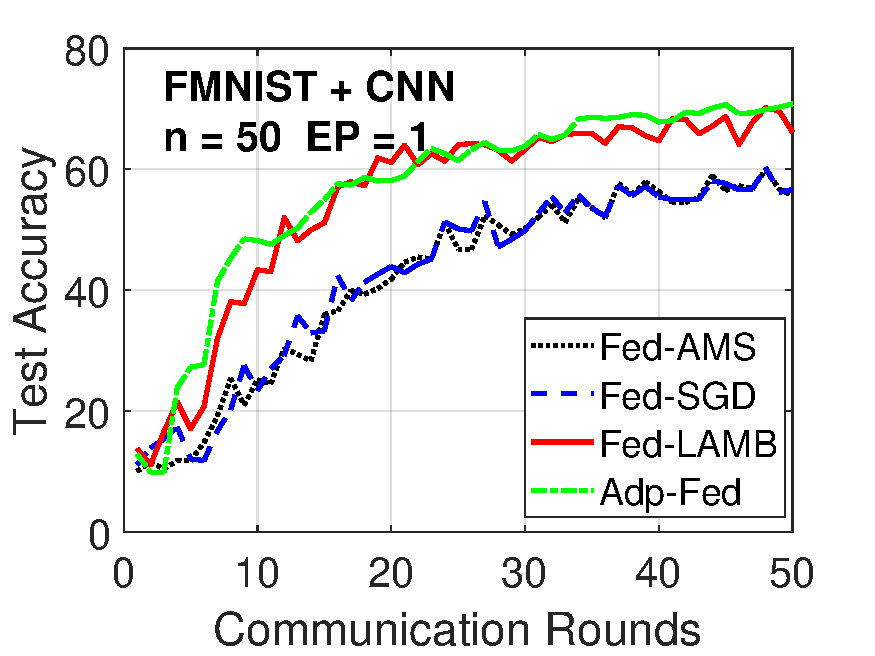
\includegraphics[width=0.25\textwidth]{new_fmnist_mnist_fig/fmnist_testerror_cnn_ep1_iid0_reddi.pdf}
        \hspace{-0.1in}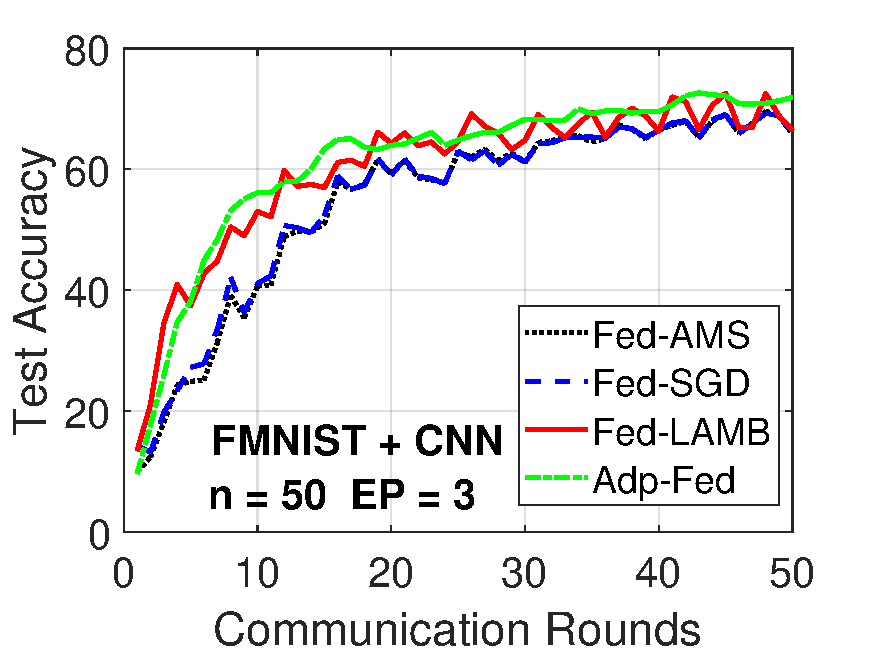
\includegraphics[width=0.25\textwidth]{new_fmnist_mnist_fig/fmnist_testerror_cnn_ep3_iid0_reddi.pdf}
        \hspace{-0.05in}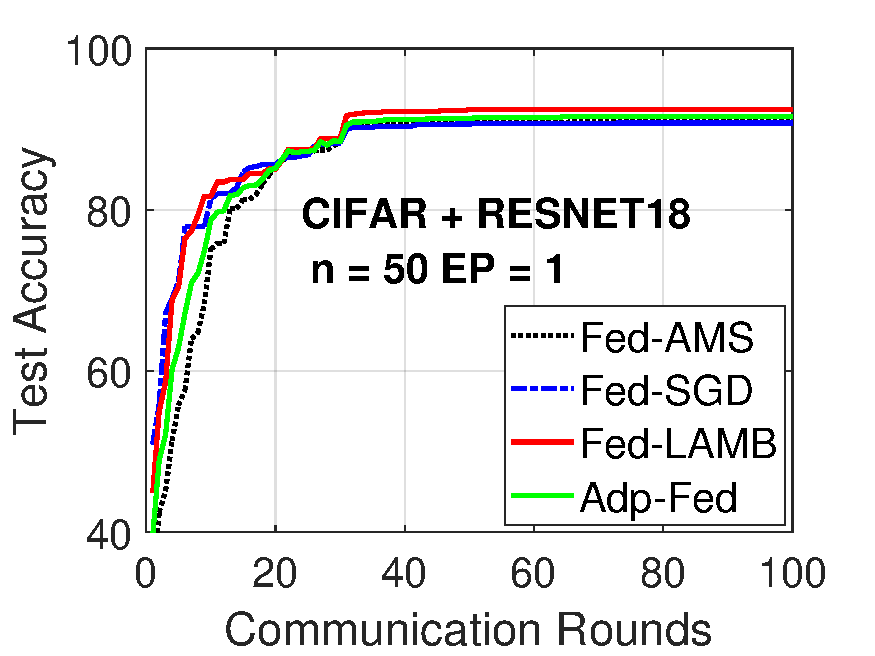
\includegraphics[width=0.25\textwidth]{new_fmnist_mnist_fig/cifar_testerror_resnet18_ep1_client2_iid0_reddi.pdf}
        \hspace{-0.1in}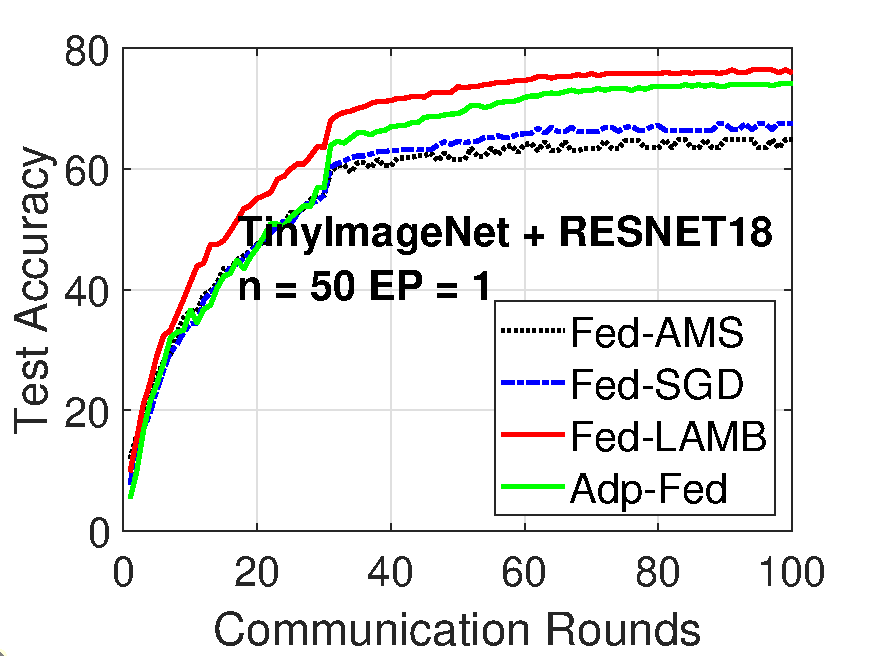
\includegraphics[width=0.25\textwidth]{new_fmnist_mnist_fig/tinyimagenet_testerror_resnet18_ep1_client2_iid0_reddi.pdf}\hspace{-0.1in}
        % \includegraphics[width=0.4\textwidth]{new_figure/tinyimagenet_testerror_resnet18_ep1_client2_iid0.eps}
        }
    \end{center}
	\caption{\textbf{non-i.i.d. data setting.} Test accuracy on FMNIST, CIFAR-10 and TinyImagenet with 50 clients.}
	\label{fig:noniidresnet18}
\end{figure}

\vspace{-0.1in}

\textbf{\textcolor{magenta}{Reviewer 15:}} We thank the reviewer for valuable comments:\vspace{-5pt}

\textbf{Discussions on the assumptions:} The smoothness assumption, the bounded variance and gradient norm are very classical in any optimization contributions (either central or federated).
Our contribution is most importantly focusing on a novel method for federated learning combined with deep neural network than on the originality of the assumptions.


% \vspace{0.1in}

% \textbf{Message to AC:} 


% Dear SPCs and ACs,

% We thank all reviewers, SPCs and ACs for their time and efforts to provide detailed and insightful comments. 
% However, we noted that two reviews are unacceptable.

% Reviewer #12 has posted an empty review (responding 'Yes' to both strengths and weaknesses).

% Reviewer #15 clearly states and admits that he/she is not familiar with the optimization field translating into a very short and superficial review where we, the authors, feel like the reviewer only expected to read keywords to make a judgment on our work (which obviously goes beyond some wording choices), see review "local minima or saddles are both expected in this terminology".

% Due to those two reviews, which are exceptionally bad, we demand a reconsideration of our paper.

% Bests,
% Authors of paper #1037

\end{document}
